\documentclass[a4paper,11pt]{article}
\usepackage{graphicx}
\usepackage{enumerate}
\usepackage[usenames, dvipsnames]{color}
\usepackage[margin=1.25in]{geometry}

\begin{document}

\begin{flushright}

\vspace{1.1cm}

{\bf\Huge Project 2}

\rule{0.25\linewidth}{0.5pt}

\vspace{0.5cm}
%Put Authors
Justin Ely
\linebreak
\newline
%Put Author's affiliations
\footnotesize{605.462 Data Visualization \\}
\vspace{0.5cm}
% Date here below
21 February, 2017
\end{flushright}

\noindent\rule{\linewidth}{1.0pt}

%%%%%%%%%%%%%%%%%%%%%%%%%%%%%%%%%%%%%%%%%%%%%%%%%%%%%%%%%%

\section{Data}
The data chosen for this project is a collection of measurements from an instrument on-board the Hubble Telescope.  During normal operations, the Cosmic Origins Spectrograph periodically measures internal characteristics of the instrument.  These can be used by scientists and engineers to monitor and diagnose issues with the instrument.  

This dataset has 201008 records with 13 variables.  Each record represents a collection of measurements and metadata from a given time sample on the instrument.  A description of each variable is given in the table below.

\begin{center}
\begin{tabular}{| l | c | l | }
  \hline	
      Variable & Type & Description  \\  \hline \hline
      id & ordinal numeric & record ID in the database \\ \hline
      obsname & nominal & name of the source observation \\ \hline
      rootname & nominal & rootname of the source observation \\ \hline
      detector & nominal & data detector label used during the observation \\ \hline
      date & ordinal numeric & date of the measurement in decimal year \\ \hline
      dark & ordinal numeric & measured dark-rate on the detector \\ \hline
      ta\_dark & ordinal numeric & measured dark-rate on the detector with no filtering \\ \hline
      latitude & ordinal numeric & spacecraft latitude during measurement \\ \hline
      longitude & ordinal numeric & spacecraft longitude during measurement \\ \hline
      sun\_lat & ordinal numeric & solar latitude during measurement \\ \hline
      sun\_lon & ordinal numeric & solar longitude during measurement \\ \hline
      temp & ordinal numeric & instrument temperature\\ \hline
      file\_id & ordinal numeric & ID of the source datafile \\ \hline
\end{tabular} \\
\end{center}

\section{Possible Questions}
This rich dataset prompts many questions which, due to its large size, are difficult to understand straight from the data.  A few possible questions include:

\begin{enumerate}
  \item Which detector has the highest dark-rate?  
  \item How are the measurements distributed in latitude and longitude? 
  \item How has the dark-rate changed over time?  
  \item Is there a correlation between dark-rate and temperature? 
  \item How many datasets have been taken for each detector?
\end{enumerate}

\section{Visualizations}

\begin{figure}[h!]
\caption{Bar chart separating dark-rate by detector and time.} 
\centering
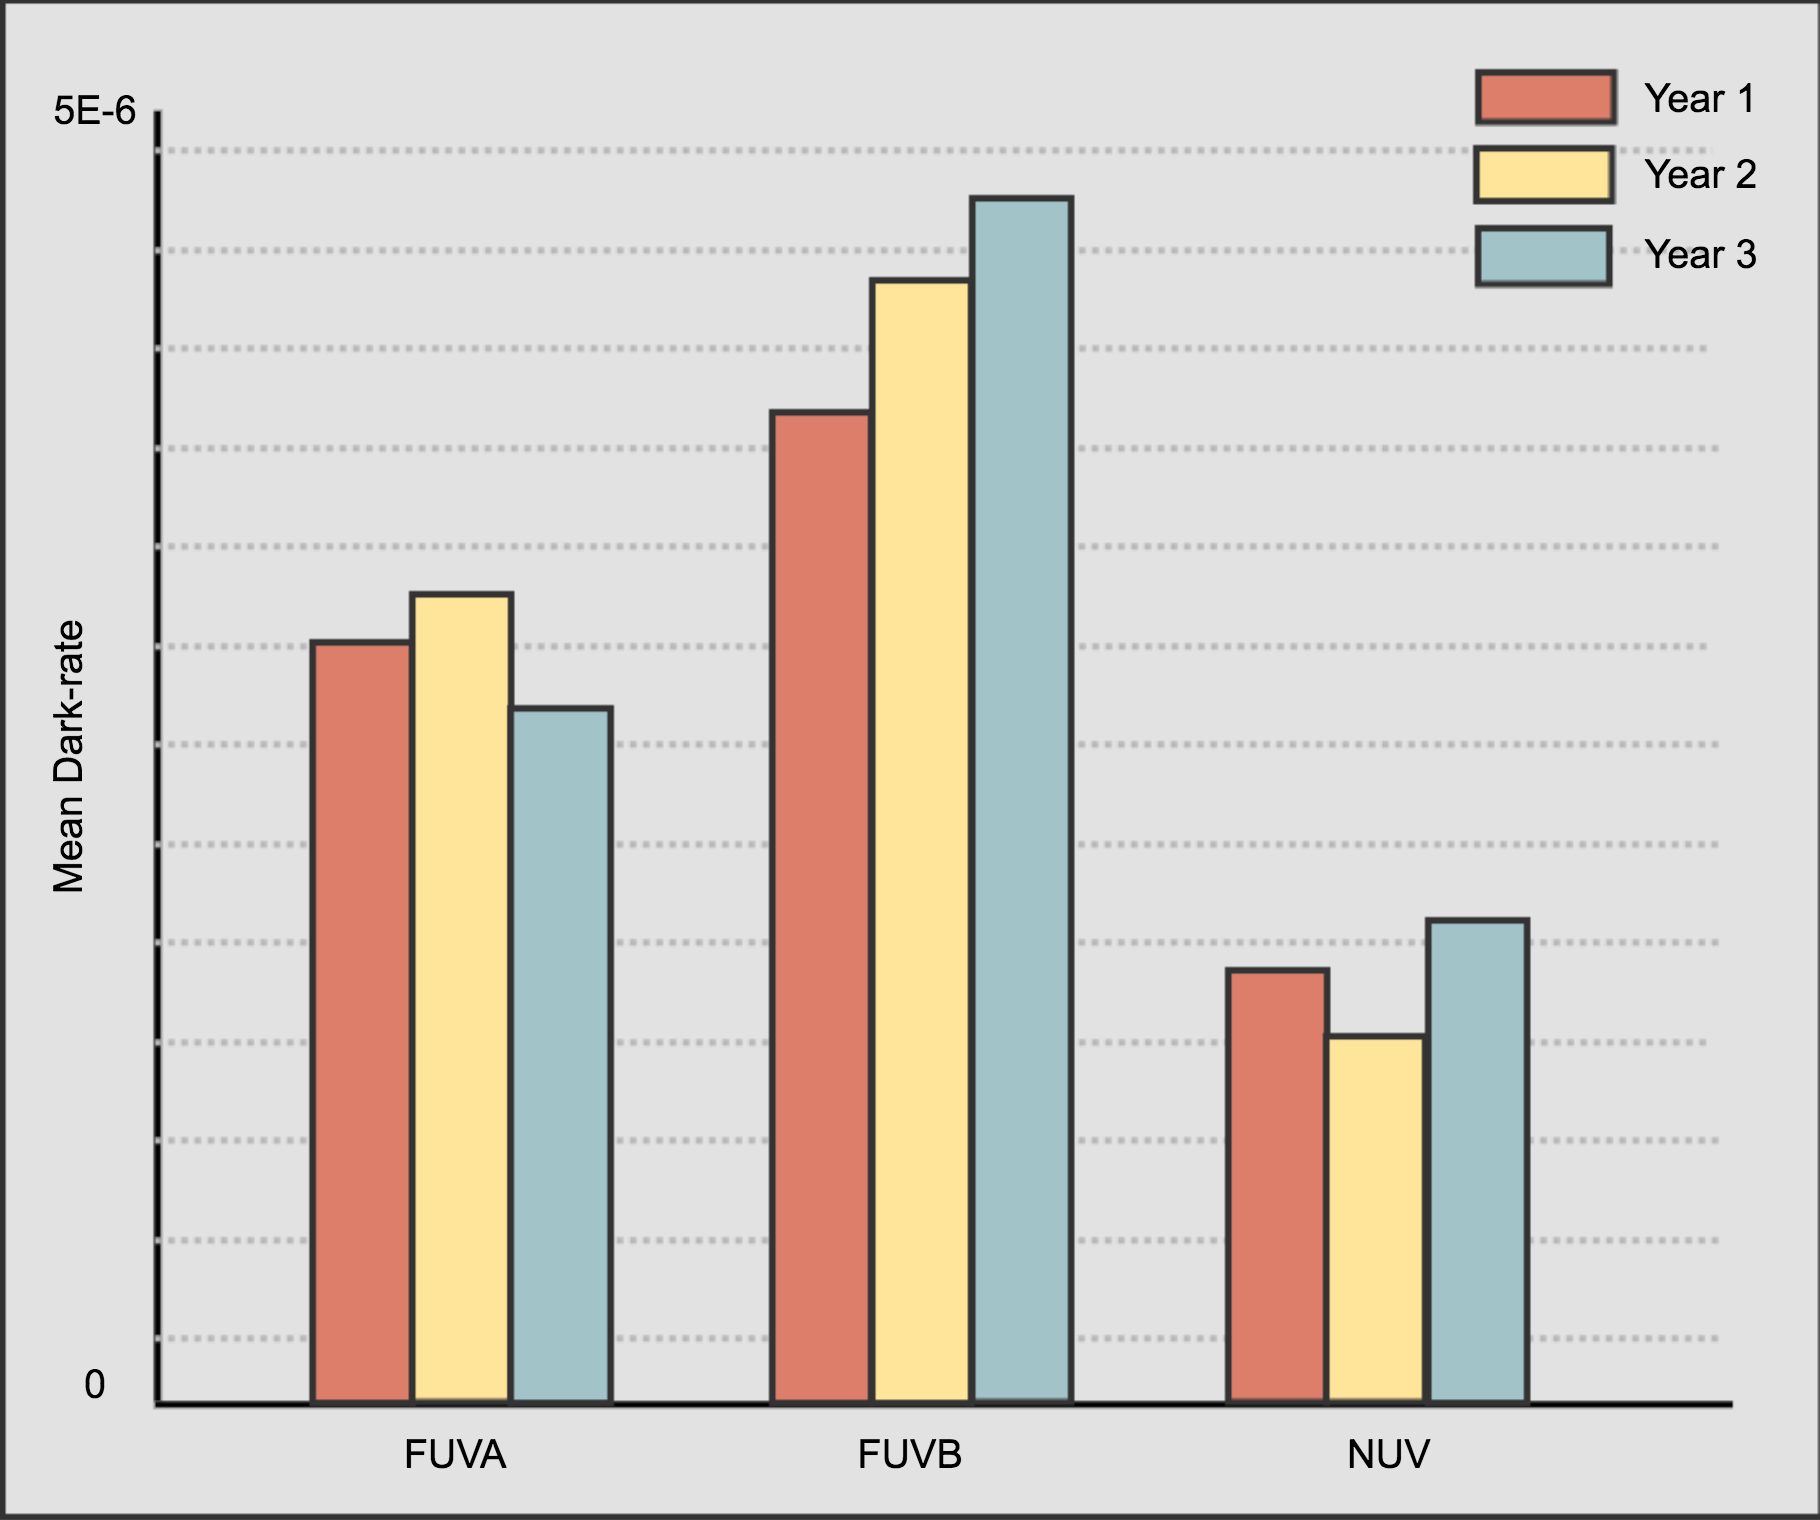
\includegraphics[width=.8\textwidth]{bars.png}
\end{figure}

To answer question 1, "Which detector has the highest dark-rate?", a simple bar chart can be used to clearly express the data.  Bars for the yearly dark-rate average for each of the 3 individual detectors would be plotted.  The yearly averages would be grouped around detector, and color-coded by year to allow quick comparison across both time and detector.  This colormap for year would not be a gradient, but instead would be distinct unique colors to make comparisons easier.  


\begin{figure}[h!]
\caption{Scatterplot showing dark-rate vs time with trendline.} 
\centering
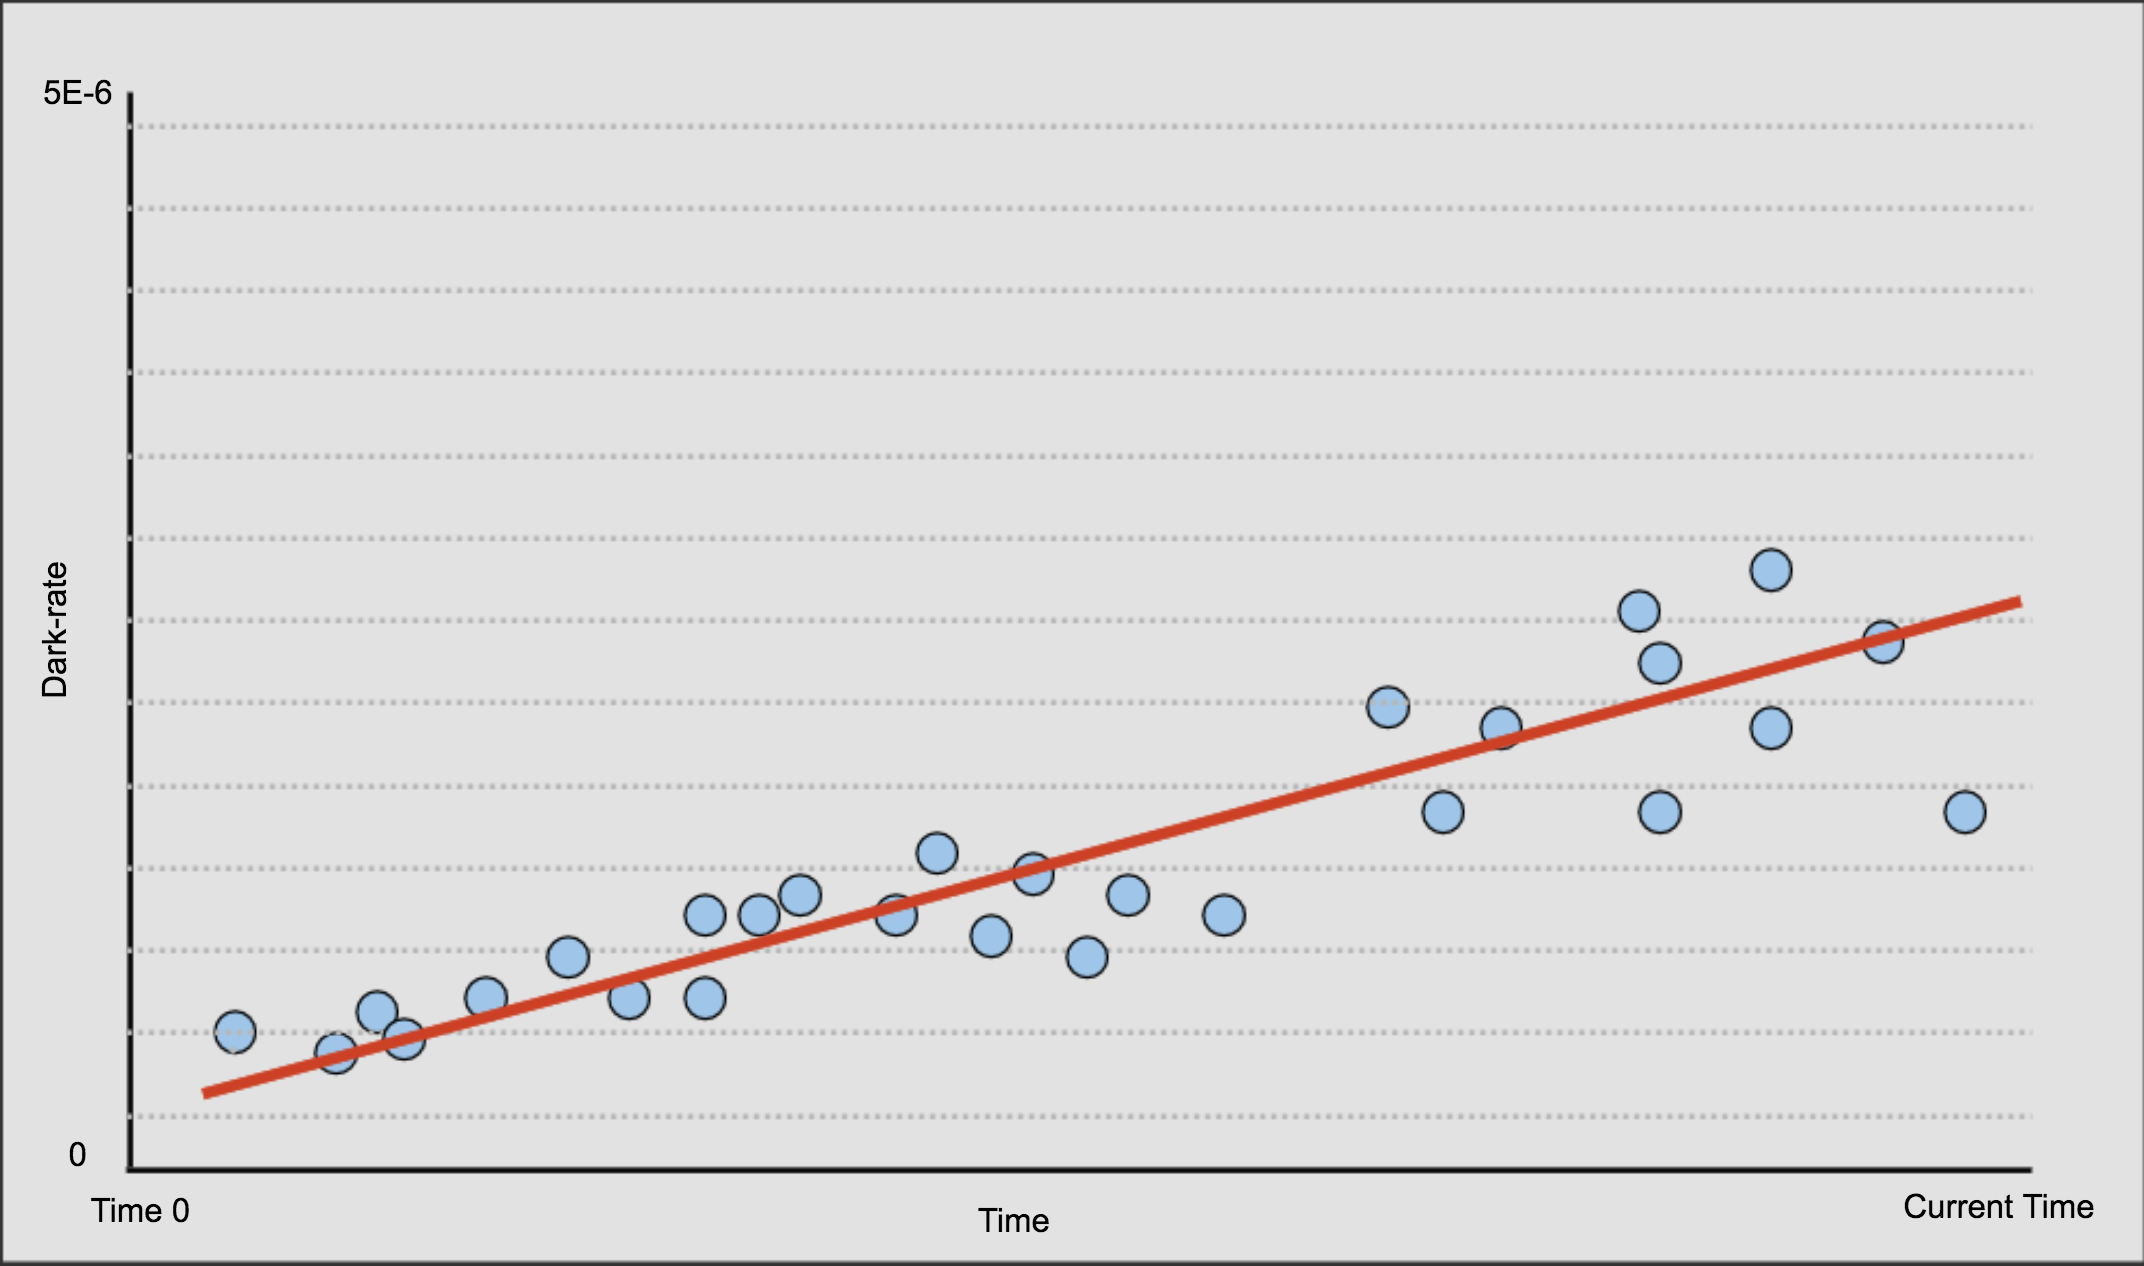
\includegraphics[width=.8\textwidth]{time.png}
\end{figure}

To answer question 3, "How has the dark-rate changed over time?", a scatter plot with trendline would help view the behavior over time.  This is a very simple visualization that only shows the data-points, in a single color, with no connecting lines.  Since the measurements are independent, connecting lines would mis-represent the data by hinting at an interpolation between measurements.  Drawn with the data would be a trendline showing the fitted behavior.  Due to the large dataset and numerous outliers, the viewer is at risk of mis-interpreting the long-term behavior.   

\begin{figure}[h!]
\caption{Dataset by dataset dark-rate scatterplot overlaid on the surface of the Earth.} 
\centering
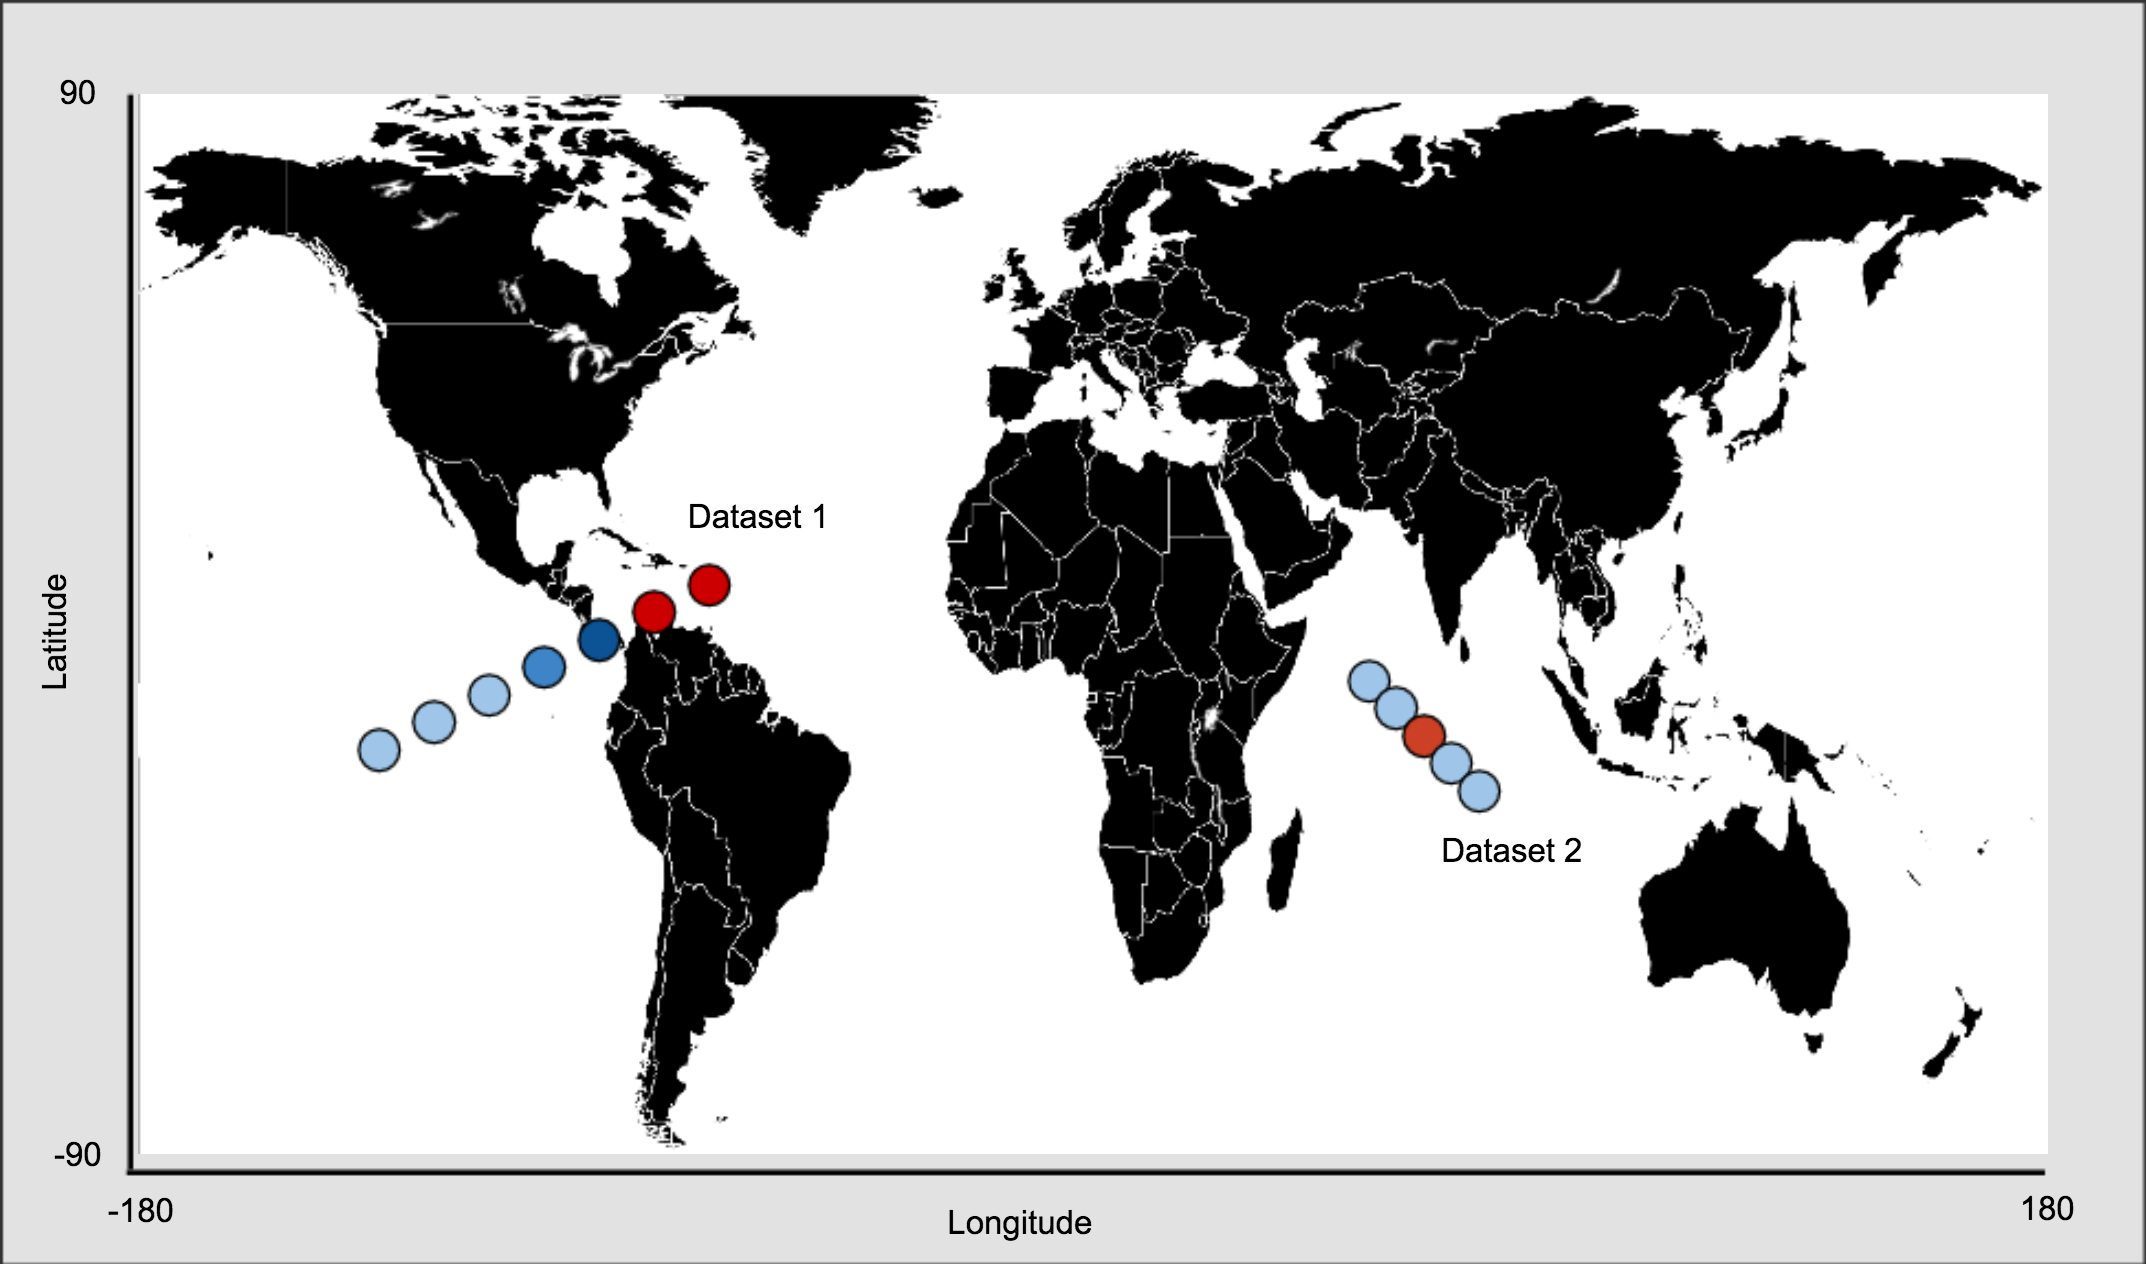
\includegraphics[width=.9\textwidth]{world.png}
\end{figure}

To answer question 2, "How are the measurements distributed in latitude and longitude?", I designed a scatterplot overlaid on a map of the earth.  Latitude and longitude make up the y and x axes.  However, since raw coordinates are hard for a viewer to associate with a geographic location, a simple map of the world would be displayed as the backdrop.  Each individual observation would then be plotted as a series of circles color-coded by dark-rate.  A text-field giving the observation name would be tied to the orbital path.  Since this representation could rapidly fill up with too many points, this visualization would need to be used on a subset or would need an interactive component to hide observations not selected by a cursor. 

%%%%%%%%%%%%%%%%%%%%%%%%%%%%%%%%%%%%%%%%%%%%%%%%%%%%%%%%%%


\end{document}
